% Straight up stealing preamble from Eli Holmes 
%%%%%%%%%%%%%%%%%%%%%%%%%%%%%%%%%%%%%%START PREAMBLE THAT IS THE SAME FOR ALL EXAMPLES
\documentclass{article}

%Required: You must have these
\usepackage{Sweave}
\usepackage{graphicx}
\usepackage{tabularx}
\usepackage{hyperref}
\usepackage{natbib}
\usepackage{pdflscape}
\usepackage{array}
\usepackage{gensymb}
\usepackage{authblk}
\renewcommand{\baselinestretch}{1.8}
%\usepackage{lineno}
%\usepackage[backend=bibtex]{biblatex}
%Strongly recommended
 %put your figures in one place
 
%you'll want these for pretty captioning
\usepackage[small]{caption}

\setkeys{Gin}{width=0.8\textwidth} %make the figs 50 perc textwidth
\setlength{\captionmargin}{30pt}
\setlength{\abovecaptionskip}{0pt}
\setlength{\belowcaptionskip}{10pt}
% manual for caption http://www.dd.chalmers.se/latex/Docs/PDF/caption.pdf

%Optional: I like to muck with my margins and spacing in ways that LaTeX frowns on
%Here's how to do that
 \topmargin -2cm 
 \oddsidemargin -0.04cm 
 \evensidemargin -0.04cm % same as oddsidemargin but for left-hand pages
 \textwidth 16.59cm
 \textheight 22.94cm 
 %\pagestyle{empty} % Uncomment if don't want page numbers
 %\parskip 7.2pt  % sets spacing between paragraphs
 %\renewcommand{\baselinestretch}{1.5} 	% Uncomment for 1.5 spacing between lines
\parindent 0pt% sets leading space for paragraphs
\usepackage[doublespacing]{setspace}
%\doublespacing

%Optional: I like fancy headers
\usepackage{fancyhdr}
\pagestyle{fancy}
\fancyhead[LO]{Soil moisture and plant phenology}
\fancyhead[RO]{2018}

%%%%%%%%%%%%%%%%%%%%%%%%%%%%%%%%%%%%%%END PREAMBLE THAT IS THE SAME FOR ALL EXAMPLES

%Start of the document
\begin{document}

% \SweaveOpts{concordance=TRUE}
\bibliographystyle{/Users/aileneettinger/citations/Bibtex/styles/ecol_let.bst}

\title{How does soil moisture interact with temperature to affect phenology?}
\begin{singlespace}

\author[1,2,a]{A.K. Ettinger}
\author[3,b]{J.S. Dukes}
\author[4,c]{M.R. Johnston}
\author[5,d]{C.R. Rollinson}
\author[1,4,6,e]{E.M. Wolkovich}

% ESA authors: Ailene K. Ettinger, Jeffrey S. Dukes, Miriam R. Johnston, Christy R.  Rollinson, and Elizabeth M. Wolkovich.
%\author[3,b]{I. Chuine}

%\author[4,5,c]{B.I. Cook}


%\author[7,e]{A.M. Ellison}

%\author[9,g]{A.M. Panetta}
%\author[11,12,i]{Y. Vitasse}

\affil[1]{Arnold Arboretum of Harvard University, Boston, Massachusetts 02131, USA}

\affil[2]{Tufts University, Medford, Massachusetts 02155, USA}

%\affil[3]{CEFE UMR 5175, CNRS, Universit\'e de Montpellier,Universit\'e Paul-Val\'ery Montpellier, EPHE IRD, Montpellier, France}

%\affil[4]{Lamont-Doherty Earth Observatory, Columbia University, Palisades, New York 10964, USA}

%\affil[5]{NASA Goddard Institute for Space Studies, New York, New York 10025, USA}

\affil[3]{Department of Forestry \& Natural Resources and Department of Biological Sciences, Purdue University, West Lafayette, Indiana 47907, USA}

%\affil[7]{Harvard Forest, Harvard University, Petersham, Massachusetts 01366, USA}

\affil[4]{Department of Organismic \& Evolutionary Biology, Harvard University, Cambridge, Massachusetts 02138, USA}

%\affil[9]{Department of Ecology and Evolutionary Biology, University of Colorado, Boulder, Colorado 80309, USA}

\affil[5]{The Morton Arboretum, Lisle, Illinois 60532, USA}

%\affil[11]{Institute of Geography, University of Neuch\^atel, Neuch\^atel, Switzerland}

%\affil[12]{Swiss Federal Institute for Forest, Snow and Landscape Research WSL, Neuch\^atel, Switzerland}

\affil[6]{Forest \& Conservation Sciences, Faculty of Forestry, University of British Columbia, Vancouver, BC, Canada}

\affil[a]{Corresponding author; email: aettinger@fas.harvard.edu; phone: 781-296-4821; mailing address: 1300 Centre Street, Boston, Massachusetts 02140, USA }

%\affil[b]{isabelle.chuine@cefe.cnrs.fr}

%\affil[c]{bc9z@ldeo.columbia.edu}

%\affil[d]{jsdukes@purdue.edu}

%\affil[e]{aellison@fas.harvard.edu}

%\affil[f]{mjohnston@g.harvard.edu}

%\affil[g]{anne.panetta@colorado.edu}

%\affil[h]{crollinson@mortonarb.org}

%\affil[i]{yann.vitasse@wsl.ch}

%\affil[j]{e.wolkovich@ubc.ca}


\date{\today}
\maketitle %put the fancy title on
%\tableofcontents %add a table of contents

%\textbf{Statement of authorship} 
%All authors conceived of this manuscript, which began at a Radcliffe Exploratory Seminar in 2016, and all authors contributed to manuscript revisions. AKE and EMW conceived of the idea for the literature review, database compilation, and related Radcliffe Exploratory Seminar. AKE compiled the datasets; AKE analyzed the data and created the figures; AKE wrote the manuscript.

%\textbf{Data Accessibility} %Data accessibility statement: The statement must confirm that, should the manuscript be accepted, the data supporting the results will be archived in an appropriate public repository such as Dryad or Figshare and the data DOI will be included at the end of the article.
%The MC3E and ExPhen databases are available at KNB \citep{ettinger2018}, along with all R code from the analyses included in this paper. (Currently, metadata are published there; the full databases and R code are available to reviewers on github.) 

%\textbf{Running title} 
%\textbf{Key words} global warming, warming experiment, microclimate, phenology, direct and indirect effects, active-warming, target temperature
\end{singlespace}


\clearpage
%%%%%%%%%%%%%%%%%%%%%%%%%%%%%%%%%%%%%%%%%%%%%%%%%%%
%\linenumbers
\begin{singlespace}
\section{Objective}
We aim to understand generally how soil moisture may affect plant phenology, and specifically if experimental effects on soil moisture in warming experiments may be responsible for the discrepency in phenology temperature sensitivity between experimental and observational studies of plant phenology. To accomplish these aims, we have three study questions:
\begin{enumerate}
\item{How do climate manipulations (target warming, precip manipulations) affect soil moisture (and temperature)?}
\item{How does soil moisture interact with temperature to affect phenology?}
\item{Does warming affect soil moisture similarly in experimental and non-experimental data?}
\end{enumerate}
\end{singlespace}
\section{How do climate manipulations affect soil moisture and temperature?}
\begin{singlespace}

\begin{enumerate}
\item{\textbf{Approach}: Use MC3E database. Fit multilevel models of soil moisture (and air temperature?) as a function of temperature and precipitation treatments.}
\noindent For this we need two equations where we evaluate the effects of experimental temperature (\textit{eT}) and experimental preciptation (\textit{eP}) treatments on soil moisture (and temperature, perhaps). There are two (or more!) possible random effects structures these models:
\begin{enumerate}

\item{Random intercepts for doy nested within year nested within site}
\begin{equation}
y_{i}=\alpha_{site[year[doy[i]]]}+ \beta_{1}eT_i+\beta_{2}eP_i+\beta_{3}eT_ieP_i+\epsilon_{i}
\end{equation}
\begin{equation}
\alpha_{site[year[doy]]}\sim N(\mu_{site[year]}, \sigma_{site[year]})
\end{equation}

\begin{equation}
\mu_{site[year]} \sim N(\mu_{sy}, \sigma_{sy})
\end{equation}

\begin{equation}
\mu_{sy} \sim N(\mu_{s}, \sigma_{s})
\end{equation}


\item{Random slopes and intercepts for site; random intercepts for doy nested within year}

\begin{equation}
y_{i}=\alpha_{site[year[doy[i]]]}+ \beta_{1 site[i]}eT_i+\beta_{2 site[i]}eP_i+\beta_{3 site[i]}eT_ieP_i+\epsilon_{i}
\end{equation}
\begin{equation}
\alpha_{site[year[doy]]}\sim N(\mu_{site[year]}, \sigma_{site[year]})
\end{equation}

\begin{equation}
\mu_{site[year]} \sim N(\mu_{sy}, \sigma_{sy})
\end{equation}

\begin{equation}
\mu_{sy} \sim N(\mu_{s}, \sigma_{s})
\end{equation}

\begin{equation}
\beta_{1 site} \sim N(\mu_{\beta1}, \sigma_{\beta1})
\end{equation}

\begin{equation}
\beta_{2 site} \sim N(\mu_{\beta2}, \sigma_{\beta2})
\end{equation}

\begin{equation}
\beta_{3 site} \sim N(\mu_{\beta3}, \sigma_{\beta3})
\end{equation}
\item{Random slopes and intercepts for site and year nested within site; random intercepts for doy. (I think we probably don't want this one...)}

\end{enumerate}

\item{\textbf{Findings}}:
\begin{enumerate}
\item{12 sites included: exps 1-5, 7-9,10 and 12-14}
\item{Target temp has a negative effect on soil moisture. (Figure \ref {fig:soilmois})}
\item{Precip treatment has a positive effect on soil moisture.(Figure \ref {fig:soilmois})}
\item{Effects vary by site. (One site, exp07, has positive effect of temperature).}
\end{enumerate}
\item{\textbf{Next steps  and questions}}:
\begin{enumerate}
\item{Fit different models for different seasonal temperatures used in Question 2?}
\item{Decide on random effects structure}
\item{Models for air temperature}
\end{enumerate}

\end{enumerate}

\section{How does soil moisture affect phenology?}
\begin{enumerate}
\item{\textbf{Approach}: Compile ExPhen database (phenology data that goes with climate data in MC3E database). Fit models with soil moisture (SM), temperature (T), and interaction to phenology data (budburst, leafout, flowering, fruiting, senesence). }
\begin{enumerate}
\item{Exclude "lud" as a phenophases becuase we have much less data for this phase compared with lod.}
\item{Excluding conifers for now.}
\end{enumerate}
\item{\textbf{Equations}Response variable (\textit{y}) is day of year of the phenological event. PRedictors are measured air temperature (\textit{T}) and soil moisture(\textit{SM}). Random effects are species (random slopes and intercepts); site and for year nested within site (random intercepts).}

\begin{equation}
y_{i}=\alpha_{sp[i],site[year[i]]}+ \beta_{1 sp[i]}T_i+\beta_{2 sp[i]}SM_i+\beta_{3 site[i]}T_iSM_i+\epsilon_{i}
\end{equation}
\begin{equation}
\alpha_{sp}\sim N(\mu_{sp}, \sigma_{sp})
\end{equation}

\begin{equation}
\mu_{site[year]} \sim N(\mu_{sy}, \sigma_{sy})
\end{equation}

\begin{equation}
\mu_{sy} \sim N(\mu_{s}, \sigma_{s})
\end{equation}

\begin{equation}
\beta_{1 sp} \sim N(\mu_{\beta1}, \sigma_{\beta1})
\end{equation}

\begin{equation}
\beta_{2 sp} \sim N(\mu_{\beta2}, \sigma_{\beta2})
\end{equation}

\begin{equation}
\beta_{3 sp} \sim N(\mu_{\beta3}, \sigma_{\beta3})
\end{equation}

\item{\textbf{Findings}}
\begin{enumerate}
\item{Air temperature (seasonal) has a negative effect on phenology for all phenophases except senescence, which has a positive effect (Figure \ref{fig:bb}). Magnitude varies among sites and species.}
\item{Moisture has a negative effect on phenology for all phenophases. Magnitude varies among sites and species. }
\end{enumerate}

\item{\textbf{Next steps and questions}}: 
\begin{enumerate}
\item{What figures to make?}
\item{How does soil moisture affect GDDcrit?}
\item Combine equations from Question 1 with equations from Questions 2 (at the annual scale) to answer: how much does 1 degree change in target temperature (\textit{eT}) affect phenology, if this were the only effect of the experiment? Similarly, how much does 50\% change in precipitation (\textit{eP}) affect phenology, if this were the only effect of the experiment? And how big a change does each make acknowledging that they both change moisture and temperature together? We can do this by plugging in different values of \textit{eT} (e.g., all 1 C, then try with all 2 C) and \textit{eP} to calculate different outcomes of moisture and temperature which we can evaluate in the equations in Question 2 to assess changes in phenology.
\item{How do we do the above with centered models?}
\end{enumerate}

\end{enumerate}
\end{singlespace}

\section{Does warming affect soil moisture and phenology similarly in experimental and non-experimental data?}
\begin{singlespace}

\begin{enumerate}
\item{Approach: Compile data from Duke (soil moisture, temp data) and Harvard Forest (soil moisture and O'Keefe phenology data). Think on best model and how to model soil moisture as a function of temperature (\textit{T}, annual? seasonal?) and precipitation (\textit{P}, annual? seasonal?). For now, \textit{y} is daily moisture across multiple years and \textit{T} is MAT and \textit{P} is percent different than mean over available time series. We use this approach to make the observational data comparable to experimental data in Question 1 above.}
\begin{equation}
y_{i}=\alpha_{doy[i]}+\beta_{1 site[i]}T_i+\beta_{2 site[i]}P_i+\beta_{3 site[i]}T_iP_i+\epsilon_{i}
\end{equation}

\begin{equation}
\alpha_{doy} \sim N(\mu_{doy}, \sigma_{doy})
\end{equation}

\begin{equation}
\alpha_{site[year]} \sim N(\mu_{sy}, \sigma_{sy})
\end{equation}

\begin{equation}
\mu_{sy} \sim N(\mu_{s}, \sigma_{s})
\end{equation}
\begin{equation}
\alpha_{sp} \sim N(\mu_{sp}, \sigma_{sp})
\end{equation}

\item{\textbf{Next steps}:We can compare \ensuremath{\beta_{1}},\ensuremath{\beta_{2}}, and \ensuremath{\beta_{3}} in experiments and observations. We may not be able to look at the \ensuremath{\beta}s themselves to do this (for instance, if data are centered).} 

\end{enumerate}
\end{singlespace}

%\section*{Abstract}

%\section* {Introduction}

%\section* {Methods}

%\section* {Results}
%\section* {Discussion}

%\section* {Conclusions}
\begin{singlespace}

\bibliography{/Users/aileneettinger/citations/Bibtex/mylibrary}
\end{singlespace}

\clearpage
\section* {Figures}
\clearpage
 \begin{figure}[h]
\centering
 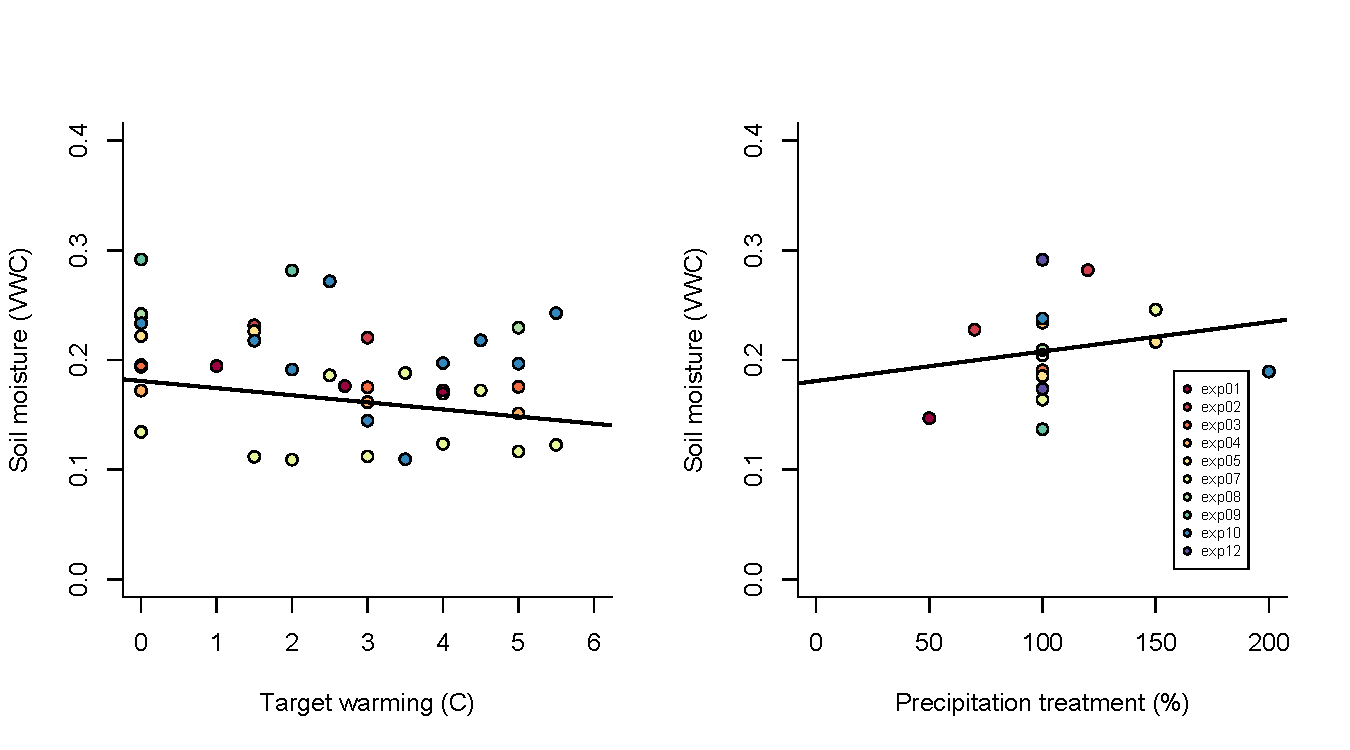
\includegraphics{/Users/aileneettinger/git/radcliffe/Analyses/soilmoisture/figures/smvstargtemp_smvspreciptreat.pdf}
 \caption{\textbf{Effects of target temperature and precipitation treatments on soil moisture.}} 
 \label{fig:soilmois}
 \end{figure}

\begin{figure}[h]
\centering
 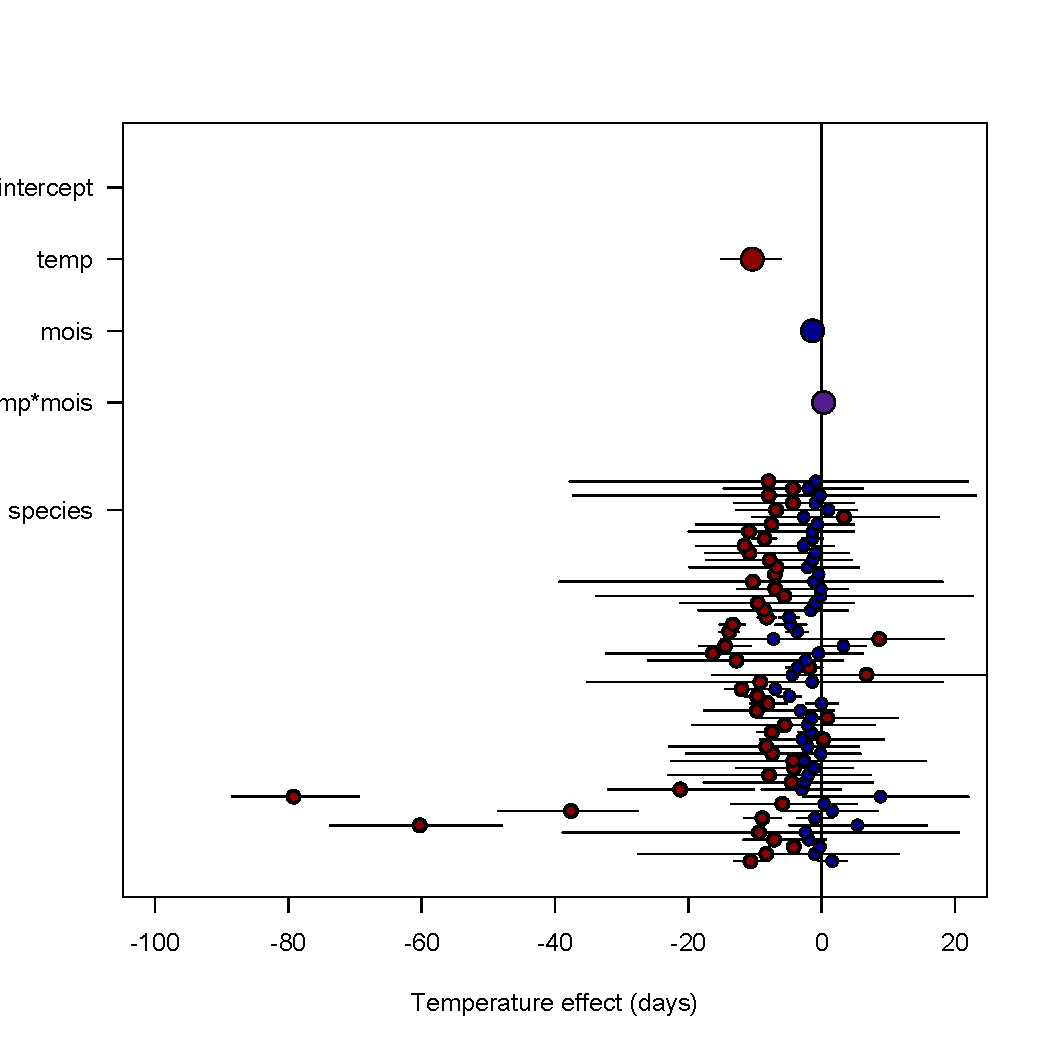
\includegraphics{/Users/aileneettinger/git/radcliffe/Analyses/soilmoisture/figures/bbdcentmodbrms.pdf}
 \caption{\textbf{Model coefficients from budburst model.}} 
 \label{fig:bb}
 \end{figure}

%%%%%%%%%%%%%%%%%%%%%%%%%%%%%%%%%%%%%%%%
\end{document}
%%%%%%%%%%%%%%%%%%%%%%%%%%%%%%%%%%%%%%%%
